%%=============================================================================
%% Proof of Concept
%%=============================================================================

\chapter{\IfLanguageName{dutch}{Proof-of-concept}{Proof-of-concept}}
\label{ch:proof-of-concept}
Na de~\nameref{ch:shortlist} kan de proof-of-concept uitgewerkt worden.
Allereerst worden de omgevingen opgezet om de uitwerking mogelijk te maken.
Hierbij volgt telkens een kleine situering van de gebruikte architectuur en gemaakte keuzes.
Daarna volgt de implementatie van de Android-app en de achterliggende service.
Tot slot worden enkele details rond reproduceerbaarheid aangehaald.
De uitgewerkte broncode kan teruggevonden worden in deze GitHub repository(TODO). % TODO github url


\section{Voorvereisten}
\label{sec:voorvereisten}
De proof-of-concept maakt gebruik van enkele bestaande tools om een werkende applicatie op te zetten.
Deze dienen vooraf ge\"{\i}nstalleerd te worden.

\subsection{Quarkus CLI}
\label{subsec:de-quarkus-cli}
De Quarkus commandline-interface tool (Quarkus CLI) kan gebruikt worden om een Quarkus-applicatie te genereren.
Deze tool kent vele installatiemogelijkheden, in deze bachelorproef werd ervoor gekozen om de package manager Chocolatey te gebruiken.
Na het installeren van deze tool wordt~\nameref{subsec:opzetten-quarkus-omgeving} mogelijk.
Het kent de bijkomende functionaliteiten om extensies toe te voegen, bij te werken of te verwijderen.
Bovendien bevordert het het updateproces van het raamwerk zelf door voorgedefinieerde acties van het Quarkus-team toe te passen tussen elke update in.
Hierdoor kan deze proof-of-concept met de steeds recentste versies van Quarkus 3 en haar extensies uitgevoerd worden.

\subsection{Java Software Development Kit}
\label{subsec:java-software-development-kit}
Naast de Quarkus CLI maakt een Quarkus applicatie ook gebruik van de Java Software Development Kit (Java SDK).
De SDK bevat een verzameling van functionaliteiten en documentatie die softwareontwikkelaars gebruiken om applicaties op te zetten.
Binnen het Java ecosysteem zijn er verschillende distributies van de Java SDK, met telkens andere implementaties van dezelfde functionaliteiten.
De voorkeur gaat in dit geval uit naar de Adoptium Eclipse Temurin distributie van Java 21, de huidige lange-termijnondersteuning versie.
Deze distributie is open-source en vereist geen betalende licentie.

\subsubsection{De Java Virtuele Machine}
Raamwerken binnen het Java ecosysteem, zoals Quarkus en Jetpack Compose, worden in de Java programmeertaal geschreven.
Ze maken daardoor gebruik van de Java SDK en de Java Virtuele Machine (JVM).
Concreet schrijven softwareontwikkelaars een applicatie bovenop deze raamwerken in programmeertalen bovenop de JVM\@, vaak is dit Java zelf.
Jetpack Compose is hier een uitzondering op waarbij softwareontwikkelaars gebruik maken van de Kotlin programmeertaal, zoals aangeraden door de ontwikkelaars achter Android.
Een build tool, in dit geval de Gradle build tool, spreekt een gespecialiseerde compiler aan om de geschreven code om te vormen naar code die leesbaarder is voor computers.
Het resultaat hiervan is Java bytecode die de JVM kan interpreteren en uitvoeren.
Android telefoons en servers gebruiken Java Virtuele Machines die ontworpen zijn voor hun interne infrastructuur en het besturingssysteem.

\subsection{Docker}
\label{subsec:docker}
Docker is een systeem vergelijkbaar met de Java Virtuele Machine.
Het bevat alle benodigdheden om software te draaien binnen gecontaineriseerde instanties die ongeacht van de infrastructuur en het besturingssysteem op een reproduceerbare manier draaien.
Hiermee ontstaat de mogelijkheid om instructies te schrijven om bepaalde diensten op te zetten op een omgeving-agnostische manier, dit in de vorm van~\textit{Docker images}.
De Docker Engine voert de instructies van de Docker images uit op een manier waarin images geen zicht hebben op andere draaiende images en de rest van het systeem.

\subsubsection{Docker Desktop}
Docker Desktop is de Docker-toepassing die gebruikt zal worden voor deze proof-of-concept.
Met deze applicatie kunnen Docker images opgezet worden om te draaien in Docker containers.
Om dit te bereiken creëert de Docker Desktop applicatie intern een virtuele machine die Linux draait waarop deze containers vervolgens draaien.

\section{Omgevingen opzetten en testen}
\label{sec:omgevingen-opzetten}
De drie lagen van de~\nameref{subsubsec:architectuur} kennen verschillende architecturele beslissingen, deze worden hieronder toegelicht.

\subsection{Opzetten Google Gemini omgeving}
\label{subsec:opzetten-google-gemini-omgeving}
Zoals verklaard in~\nameref{ch:shortlist} biedt Google Vertex AI allerlei taalmodellen ter beschikking voor Google Cloud gebruikers.
Een omgeving opzetten is triviaal, een gebruiker hoeft daarbij enkel een Googleaccount en project aan te maken op Google Cloud.
Daarna kiest de gebruiker ervoor om de Vertex AI-mogelijkheden en bijhorende taalmodellen aan te zetten.
Voor prototypes is het mogelijk om € 280 aan krediet aan te vragen, waarmee nieuwe klanten de functionaliteiten van Gemini gratis kunnen uitproberen.
Ten slotte hoort de server toegang te krijgen tot Vertex AI, dit kan door het volgen van de \textit{Set up Application Default Credentials} handleiding voor lokale ontwikkelingsomgevingen\footnote{De handleiding kan \href{https://cloud.google.com/docs/authentication/provide-credentials-adc#local-dev}{hier} geraadpleegd worden}.

\subsection{Opzetten van de Quarkus omgeving}
\label{subsec:opzetten-quarkus-omgeving}
De Quarkus commandline-interface tool Quarkus CLI maakt het genereren en beheren van Quarkus-applicaties mogelijk.
Gezien we gebruik willen maken van het Kotlin-ecosysteem om consistent te blijven met onze Android-app zal de Kotlin extensie toegevoegd worden samen met enkele andere Quarkus-extensies:
\begin{itemize}
    \item \textbf{Hibernate ORM Panache Kotlin} zal de gegevens van de gebruikers en personal trainer opslaan in de databank op een Kotlin-gerichte wijze.
    \item \textbf{Java Database Connectivity (JDBC)} verzorgt de connectie met de databank zelf.
    JDBC haalt de inloggegevens van de databank op uit de application.properties bestand van de Quarkus-app.
    Als deze niet gedefinieerd zijn, dan zal Quarkus zelf een databank opstarten in een Docker-container en dit doorgeven aan JDBC\@.
    \item \textbf{Hibernate Validator} vergemakkelijkt het valideren van binnenkomende data van gebruikers.
    Langs deze weg verplicht de API de gebruiker om een foto mee in het verzoek te versturen.
    \item \textbf{LangChain4j}, tenslotte, maakt de communicatie met de Google Gemini-omgeving mogelijk.
\end{itemize}
Met de voornoemde specificaties in het achterhoofd gehouden kan deze commando uitgevoerd worden om het Quarkus-project op te zetten:
\begin{listing}[H]
    \begin{minted}[breaklines]{sh}
quarkus create app mauricecantaert:bachelorproef-ti-quarkus \
    --extensions=kotlin,rest,rest-jackson,rest-multipart,hibernate-orm-panache-kotlin,hibernate-validator,jdbc-mariadb,quarkus-langchain4j-core \
    --gradle-kotlin-dsl
    \end{minted}
    \captionof{listing}{\IfLanguageName{dutch}{Commando om het Quarkus project met bijhorende extensies en configuratie te genereren}{Command to generate the Quarkus project with extensions and configuration}}
\end{listing}

\subsubsection{De werking van een Quarkus API}
\label{subsubsec:werking-api}
De achterliggende service is geschreven volgens de principes van de REST-architectuur.
REST, of Representational State Transfer, is een vorm van een Application Programming Interface (API) dat het communiceren tussen apparaten via het internet standaardiseert~\autocite{Doglio2018}.
De voornaamste vereiste van een REST-applicatie is het behandelen van elk verzoek als nieuwe taak die telkens reproduceerbaar is.
Daaropvolgende verzoeken kennen geen geschiedenis van voorgaande verzoeken, waardoor het noodzakelijk is om steeds alle data mee te geven in één verzoek.

\subsubsection{Het aanspreken van functionaliteiten binnen de Quarkus API}
Elke bron, of type verzoek, krijgt volgens de REST-architectuur een Uniforme Bronidentificatie (URI) die gebruikt kan worden om de achterliggende dienst aan te spreken.
Deze Quarkus API kent daarmee twee bronnen, één voor de gebruikers en één voor personal trainers.
Gebruikers krijgen daarbij de mogelijkheid om fitnessinstrumenten te detecteren en daarvoor suggesties te laten genereren.
Personal trainers krijgen zicht op de geschiedenis van gebruikers en kunnen de suggesties bijsturen waar nodig.
Concreet spreekt de Android-app de achterliggende service aan met de gewenste URI's.

\subsection{Opzetten Jetpack Compose Android-app omgeving}
\label{subsec:opzetten-jetpack-compose-android-app}
Cliënten horen de mogelijkheid te hebben om de opgezette Quarkus applicatie op te roepen vanuit een Android applicatie.
Gebruikers kiezen daarvoor om een nieuwe foto te maken of een bestaande te selecteren uit de galerij van hun telefoon.
Het Android besturingssysteem verplicht applicaties om hiervoor eerst toestemming te vragen aan de gebruiker, wat geïmplementeerd zal worden door gebruik te maken van het bestaande proces dat het besturingssysteem beschikbaar stelt.
Tot slot zal Retrofit, een bestaande oplossing om REST-verzoeken te versturen en ontvangen, de connectie met de Quarkus dienst behandelen.
Android Studio, de geïntegreerde ontwikkelaarsomgeving voor ontwikkelaars op het Android platform, biedt een template aan voor het genereren van een Android project.
Deze maakt standaard gebruik van het Gradle bouwsysteem, wat de Quarkus api tevens ook gebruikt.

\subsection{Gemini AI testen}
\label{subsec:gemini-ai-testen}
Vertex AI biedt een test interface vergelijkbaar aan de werking van Langchain4j.
Dit is belangrijk om de eerste stap in het gebruiksverloop van klanten te testen.
Als het gebruik hiervan een ongunstig resultaat zou opleveren, betekent dit dat het gebruikte taalmodel ongepast is voor deze proof-of-concept.
Hierna volgen enkele testen van het Gemini 1.5 Pro platform, de resultaten worden gegoten in een vooraf gedefinieerde JSON-formaat.
Het model krijgt de instructie om een schatting te maken voor onzekere eigenschappen, zoals wanneer het gewicht niet duidelijk vermeld.
In elke test wordt gekozen voor een afbeelding gemaakt met een andere telefoon om verschillende gebruikers te simuleren.

\subsubsection{Eerste test}
De eerste afbeelding~\ref{fig:test-een} bevat enkel de bovenkant van een dumbbell, de dumbbell zelf is dus niet triviaal te detecteren door het model.
Het gewicht daarentegen is wel duidelijk zichtbaar, namelijk 16 pond.
Gemini geeft een gunstig resultaat en detecteert het onderwerp en het gewicht:
\begin{listing}[H]
    \begin{minted}[breaklines]{json}
{
    "name": "DUMBBELL",
    "type": "FREE_WEIGHT",
    "weight": 16,
    "weight_measurement": "LBS",
    "unknown_fields": []
}
    \end{minted}
    \captionof{listing}{\IfLanguageName{dutch}{Resulterende JSON-data van de eerste computer visie test.}{Resulting JSON-data from the first computer vision test.}}
\end{listing}

\begin{figure}[H]
    \begin{center}
        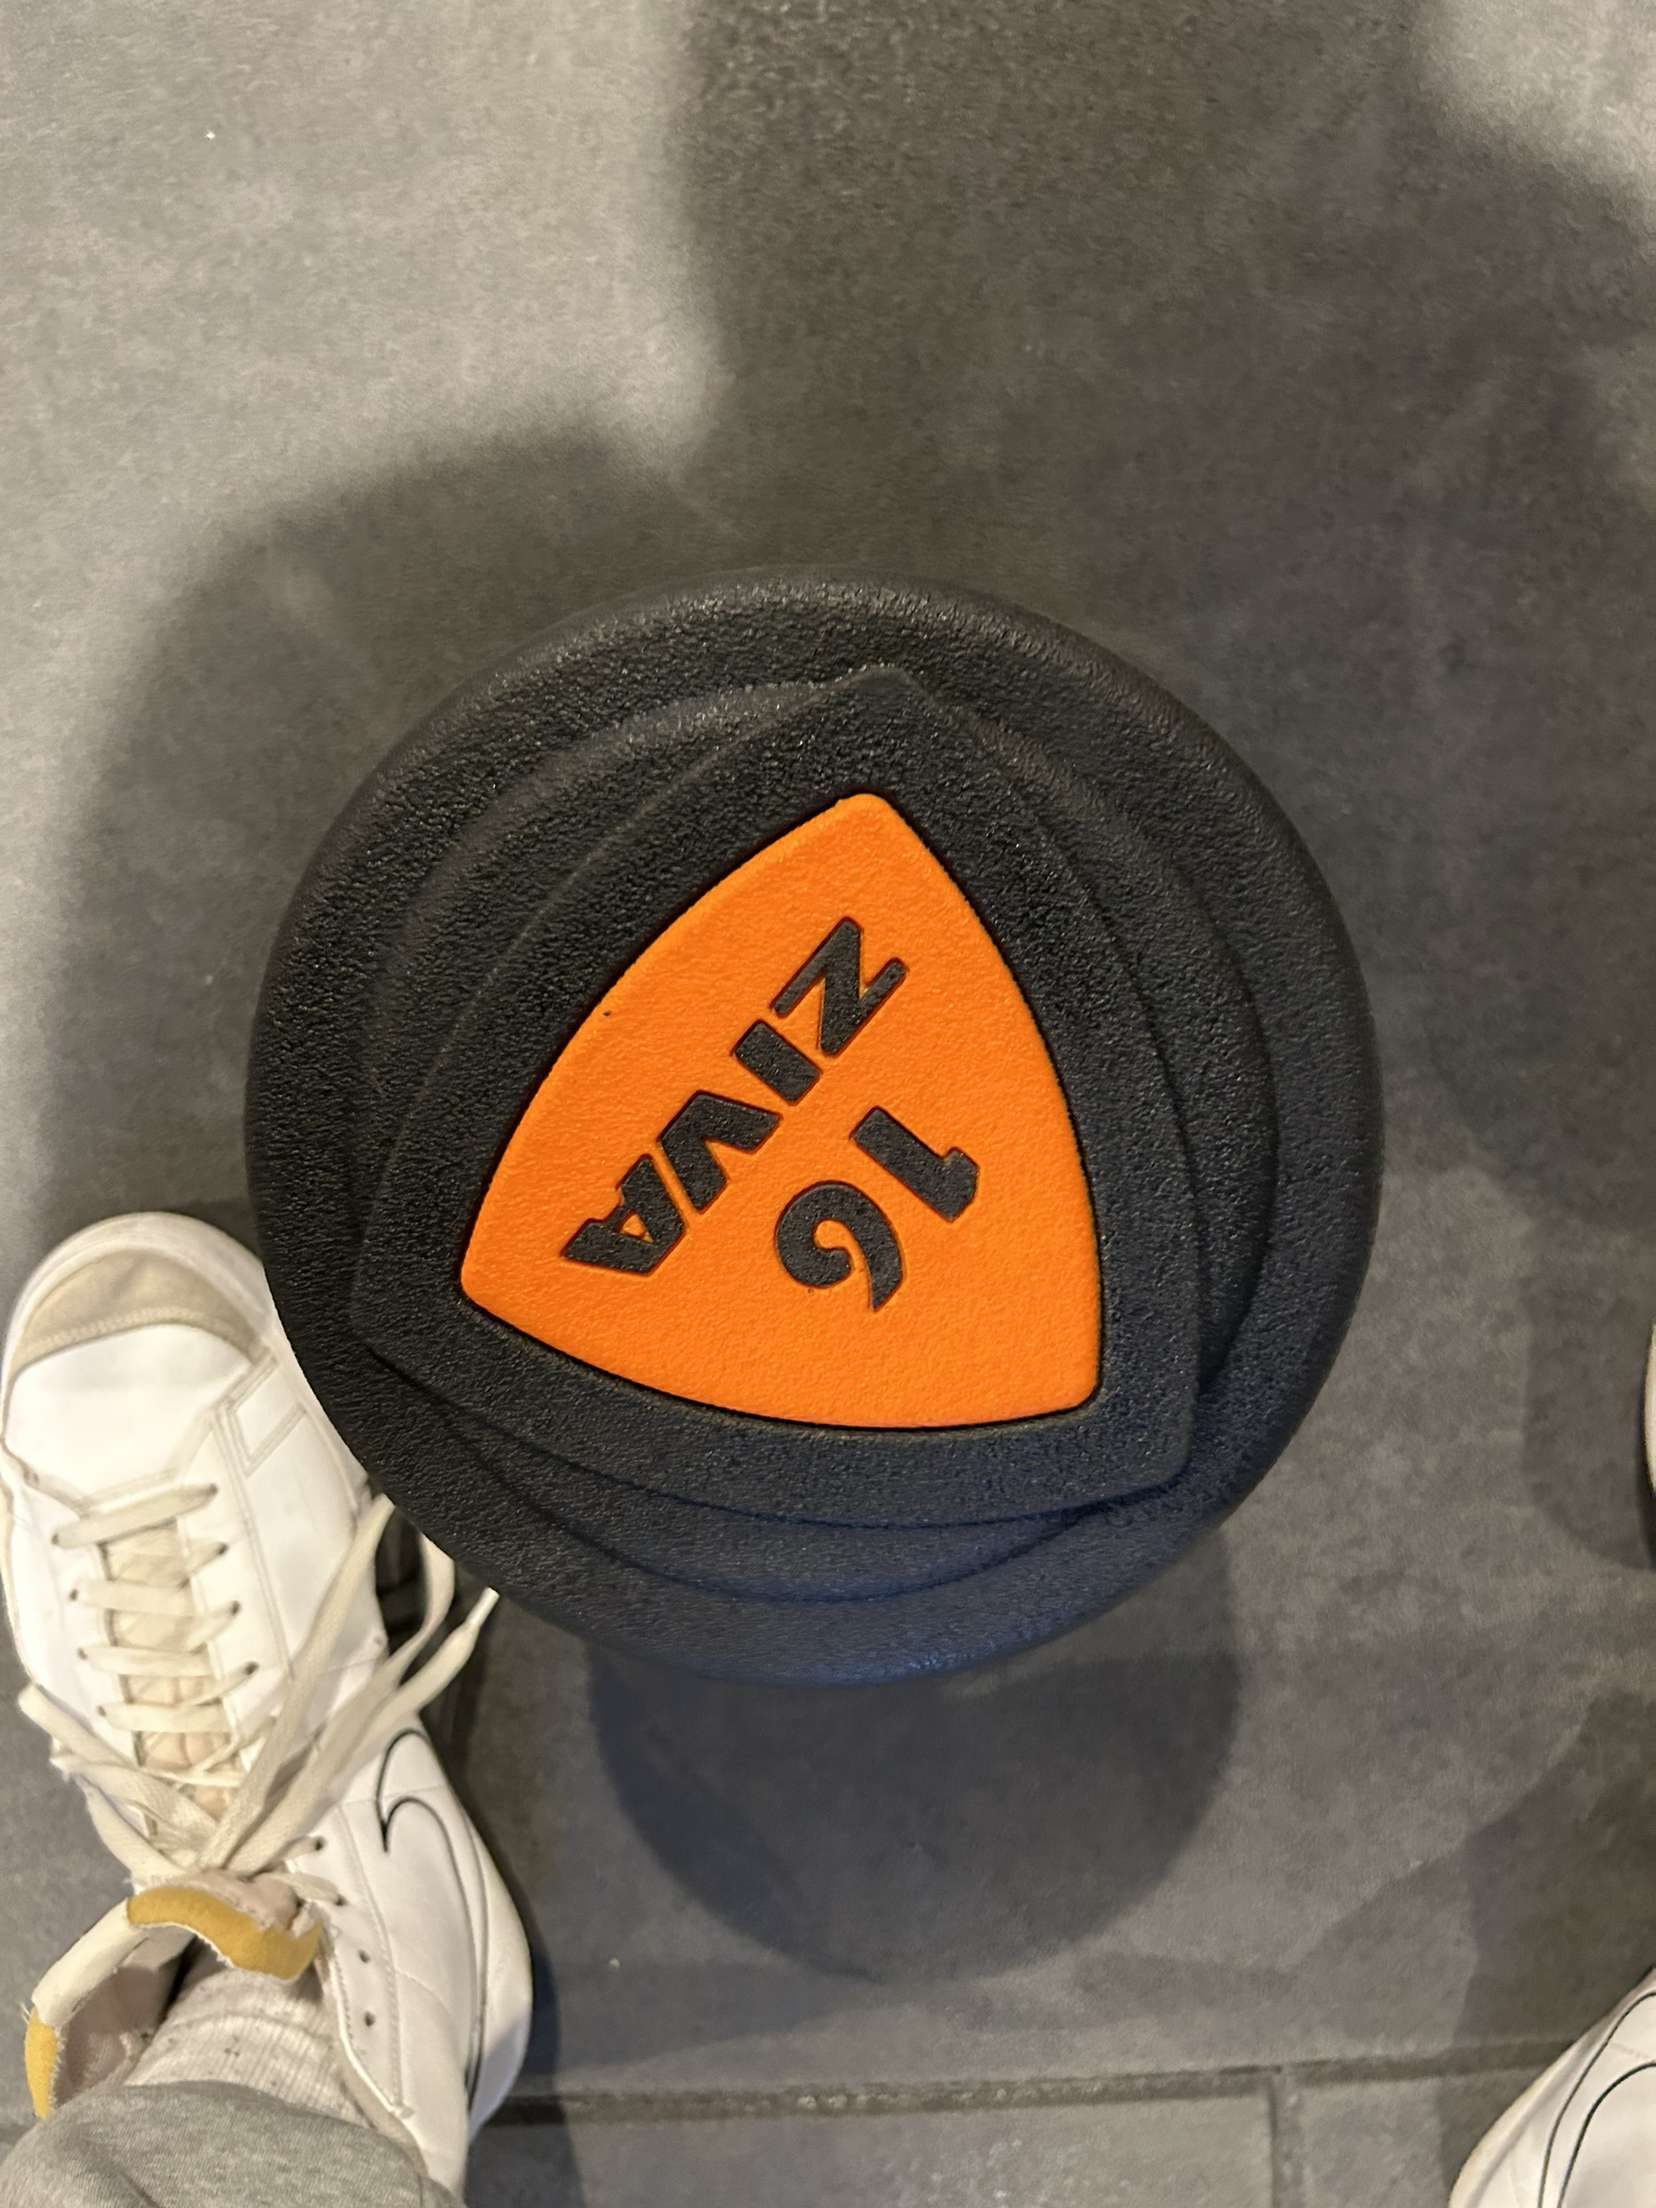
\includegraphics[scale=0.1]{images/prompt1-image}
        \caption{De bovenkant van een 16 pond dumbbell, de foto werd genomen met een Apple iPhone 14.}
        \label{fig:test-een}
    \end{center}
\end{figure}

\subsubsection{Tweede test}
Voor de tweede test bevat afbeelding~\ref{fig:test-twee} de zijkant van twee dumbbells.
Echter is het gewicht, 8 kilogram, in dit geval minder duidelijk zichtbaar,
Gemini geeft wederom een gunstig resultaat en detecteert zowel het onderwerp als het gewicht:
\begin{listing}[H]
    \begin{minted}[breaklines]{json}
{
    "name": "DUMBBELL",
    "type": "FREE_WEIGHT",
    "weight": 8,
    "weight_measurement": "KG",
    "unknown_fields": []
}
    \end{minted}
    \captionof{listing}{\IfLanguageName{dutch}{Resulterende JSON-data van de tweede computer visie test.}{Resulting JSON-data from the first computer vision test.}}
\end{listing}

\begin{figure}[H]
    \begin{center}
        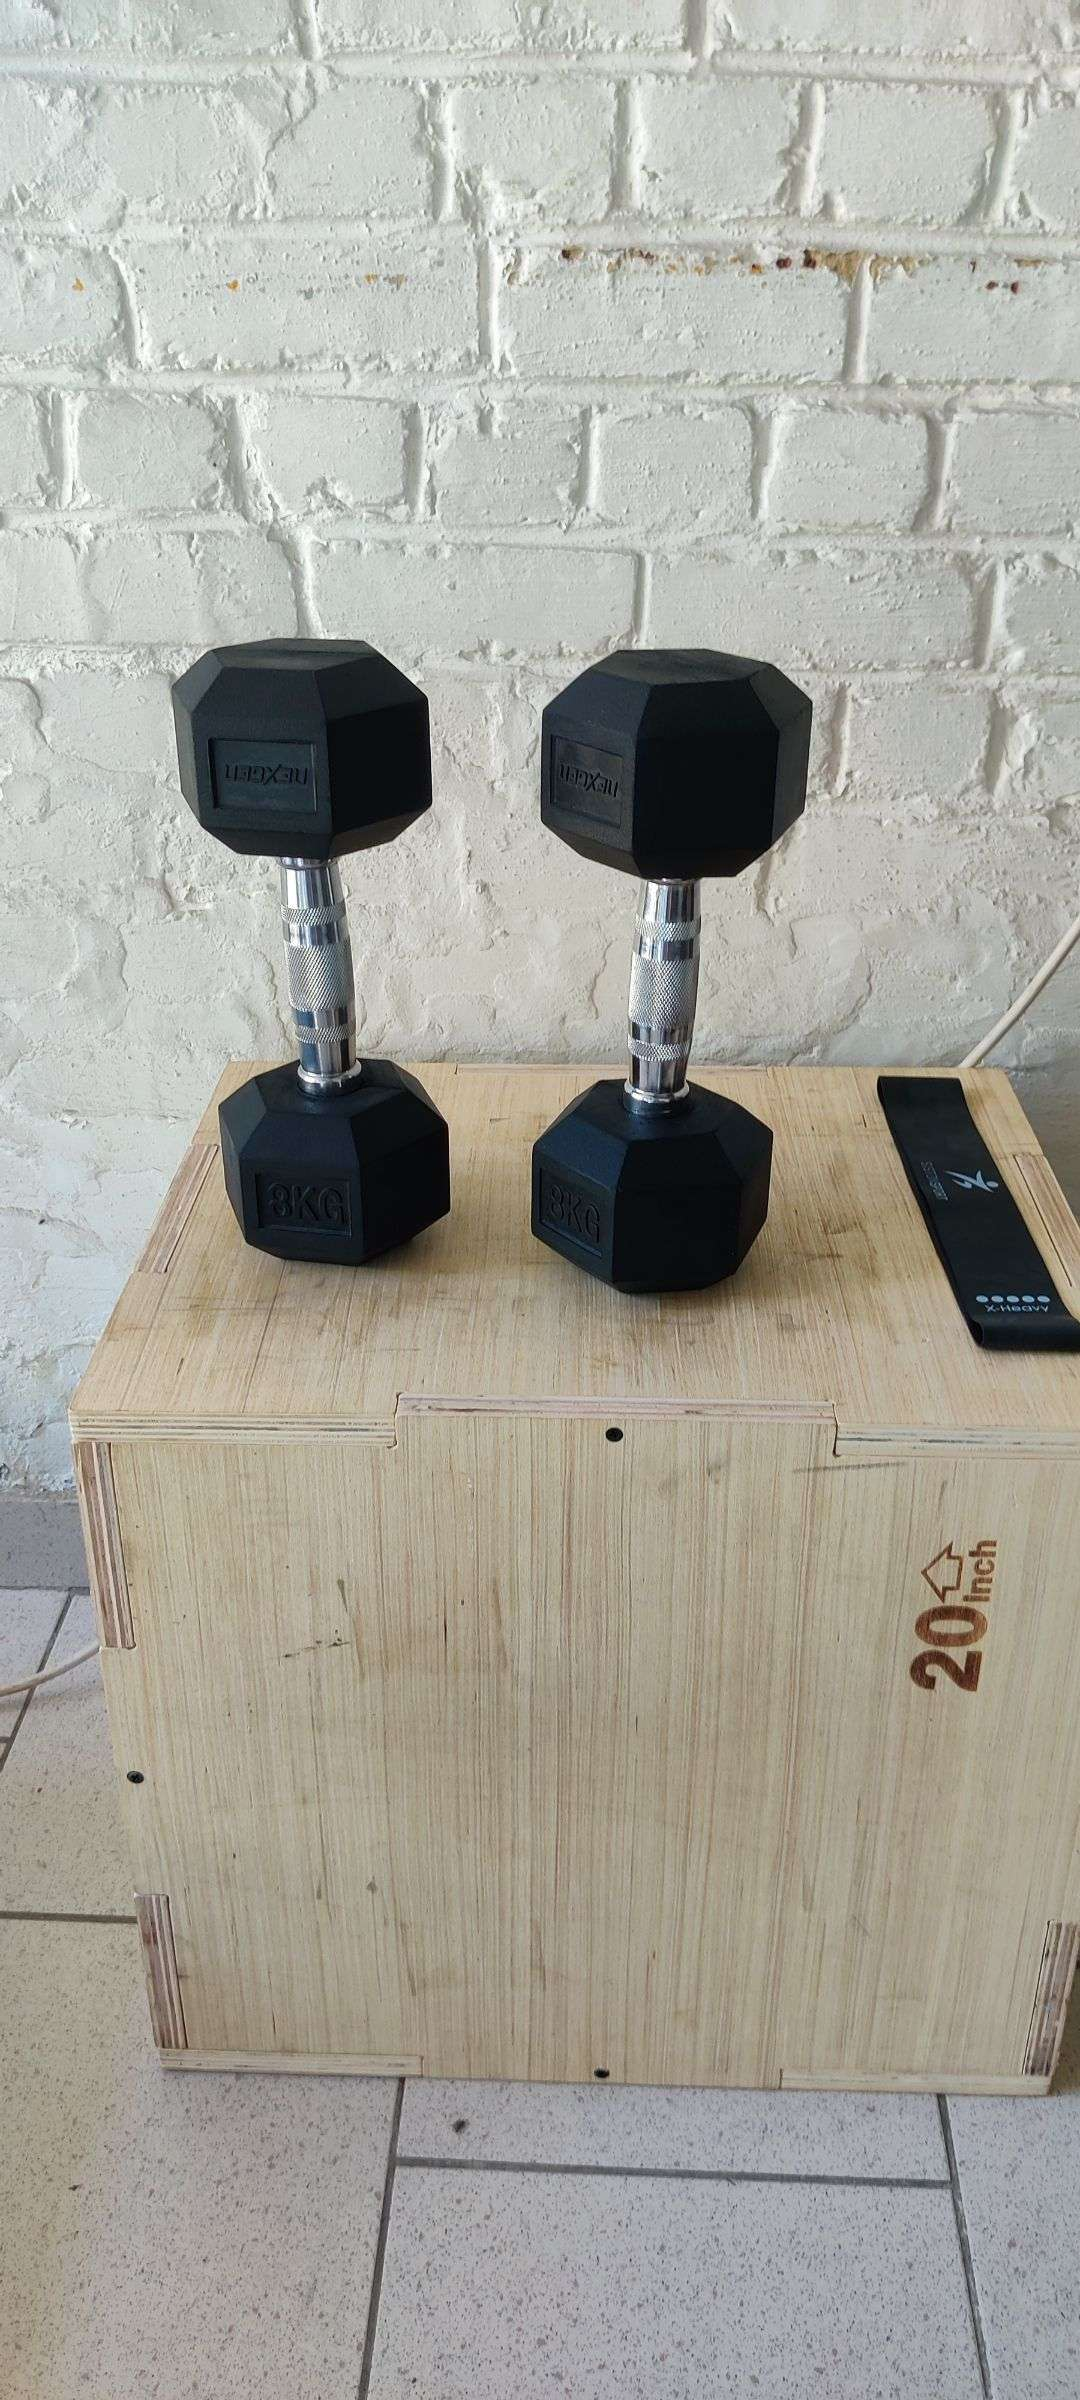
\includegraphics[scale=0.20]{images/prompt2-image}
        \caption{De zijkant van twee 8 kilogram dumbbells, de foto werd genomen met een OnePlus 8T.}
        \label{fig:test-twee}
    \end{center}
\end{figure}

\subsubsection{Laatste test}
Ten slotte bevat de laatste test afbeelding~\ref{fig:test-drie} met een dumbbell met een gewicht van 5 kilogram, dit gewicht staat echter niet beschreven op het voorwerp.
Gemini geeft hierbij een correcte inschatting van het gewicht, maar deelt mee dat het slechts om een inschatting gaat:
\begin{listing}[H]
    \begin{minted}[breaklines]{json}
{
    "name": "DUMBBELL",
    "type": "FREE_WEIGHT",
    "weight": 5,
    "weight_measurement": "KG",
    "unknown_fields": [
        "weight"
    ]
}
    \end{minted}
    \captionof{listing}{\IfLanguageName{dutch}{Resulterende JSON-data van de laatste computer visie test.}{Resulting JSON-data from the first computer vision test.}}
\end{listing}

\begin{figure}[H]
    \begin{center}
        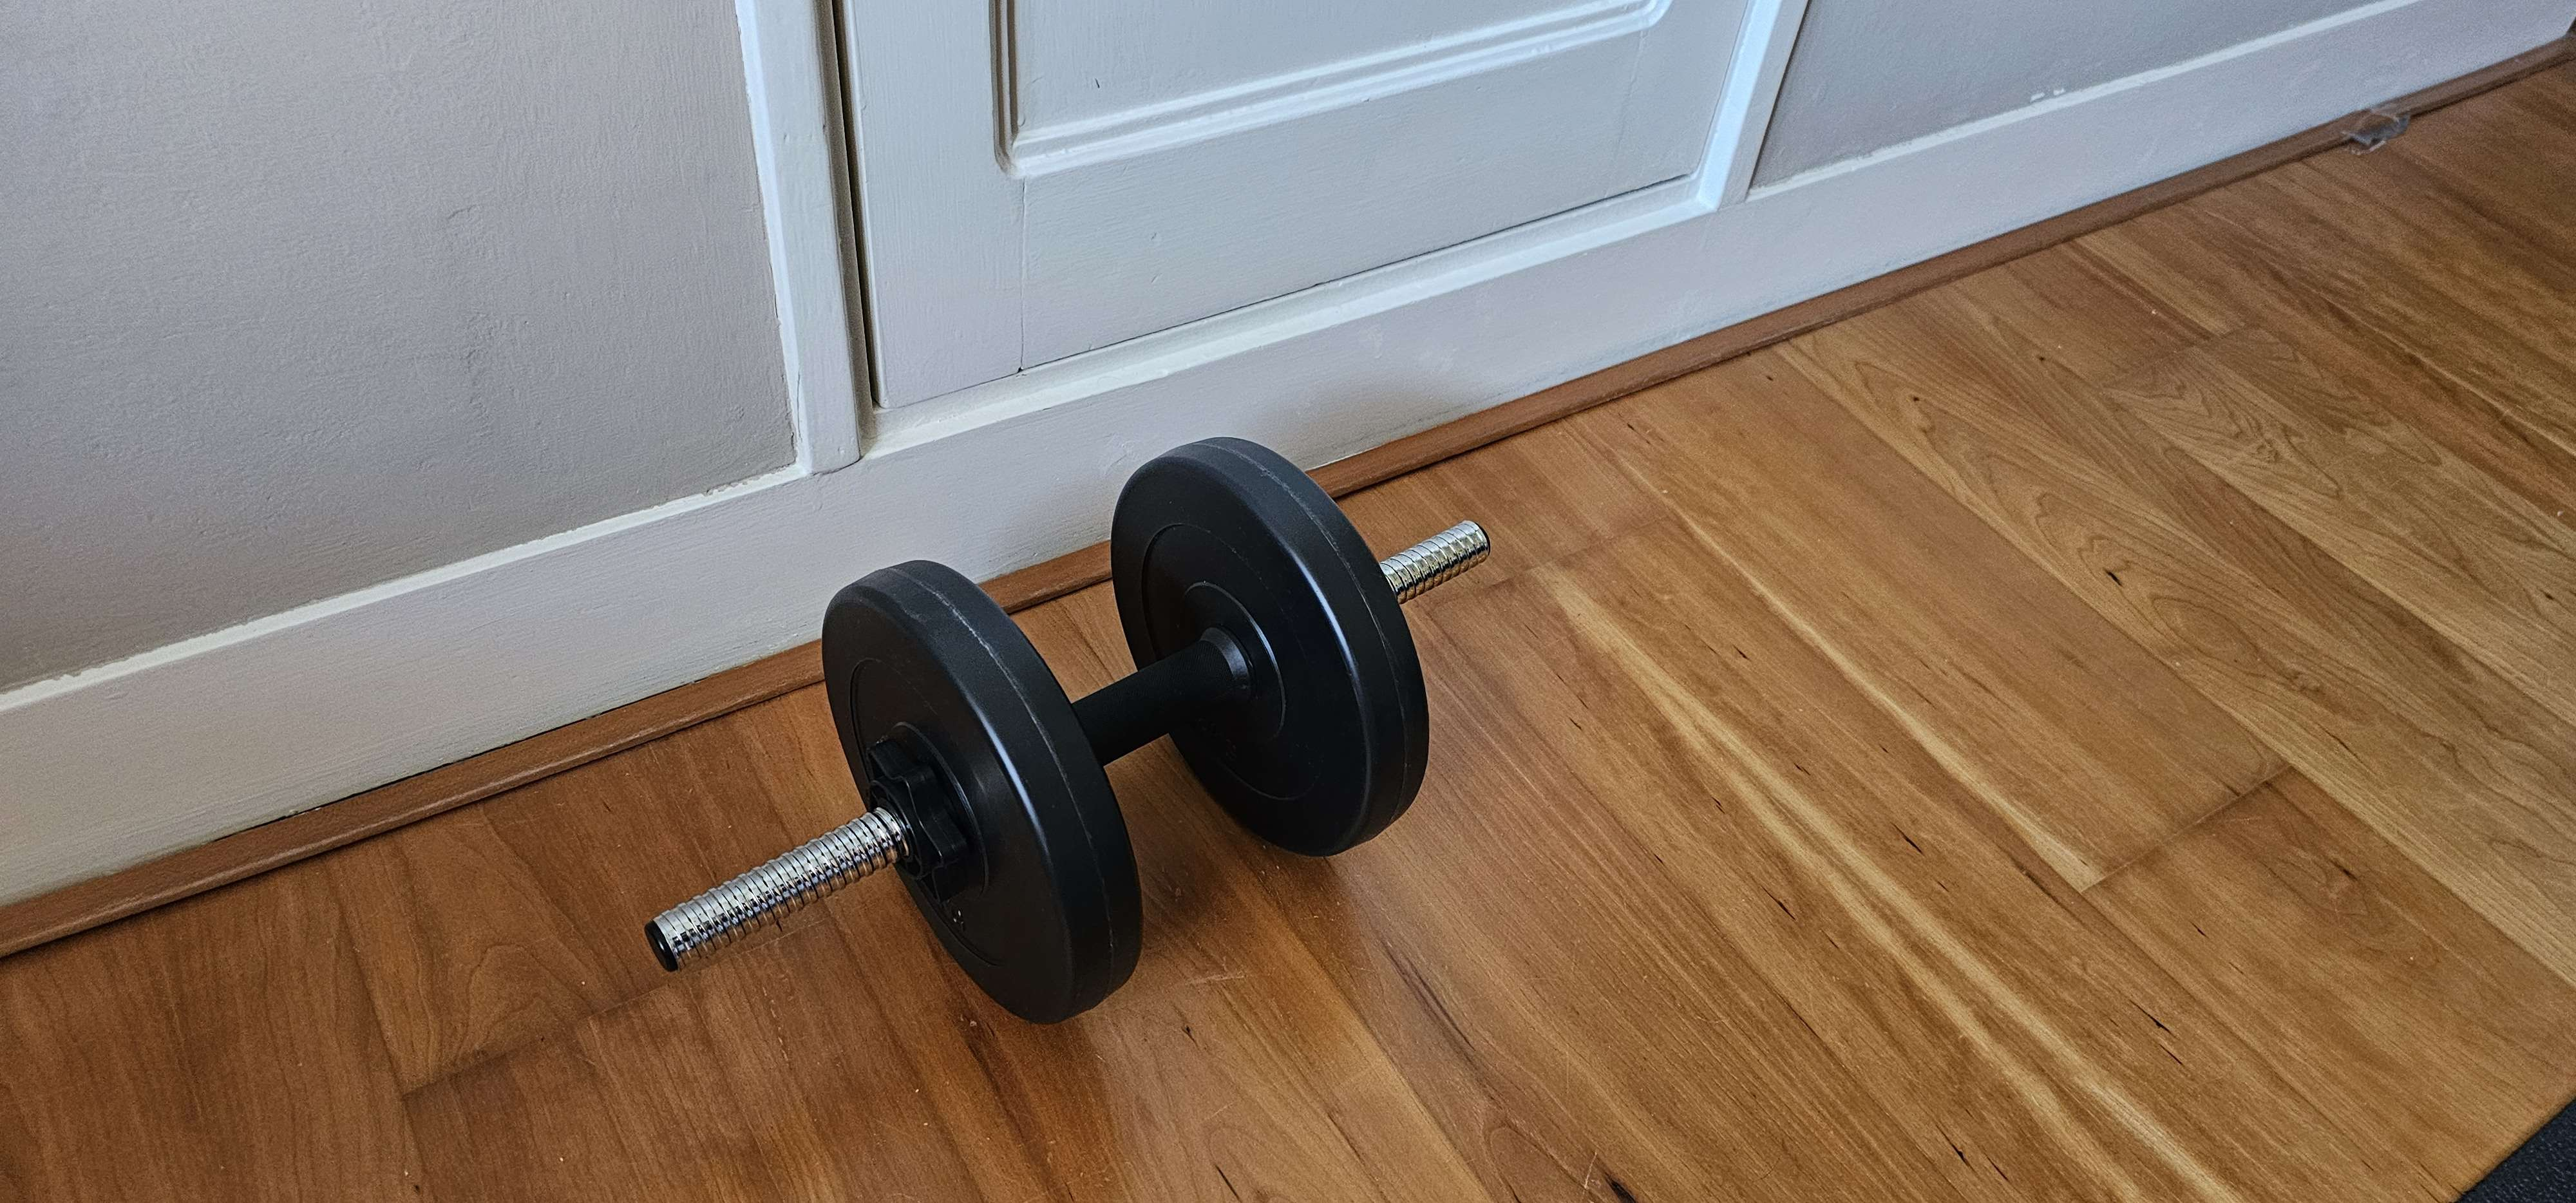
\includegraphics[scale=0.11]{images/prompt3-image}
        \caption{Een zijaanzicht van een 5 kilogram dumbbell, de foto werd genomen met een Samsung S23 Ultra.}
        \label{fig:test-drie}
    \end{center}
\end{figure}

\section{Functionaliteiten uitwerken}
\label{sec:functionaliteiten-uitwerken}
De resultaten uit de vorige stap bewijzen de mogelijkheden van het Gemini-platform, hiermee ontstaat de zekerheid dat de proof-of-concept hier verder op zal kunnen bouwen.
Eerst volgt de opzet van het domeinmodel in de achterliggende service, dit dient om de historiek van de gebruiker bij te kunnen houden in de databank.
Daarna volgt een uitwerking van de bronnen die de gebruiker en de personal trainer zal kunnen oproepen om de functionaliteiten te gebruiken.
De gebruiker zal deze bronnen kunnen oproepen door middel van een kleine Android-app, wat in de laatste stap opgezet wordt.
Een demo geeft het zicht op de bereikte functionaliteiten en de resultaten, wat besproken zal worden in de volgende sectie.

\subsection{Domeinmodel opzetten}
\label{subsec:domeinmodel-opzetten}
De achterliggende service hoort de historiek van de gebruiker bij te houden zodat de coach deze op elk moment hoort te kunnen raadplegen.
Om dit te bereiken zullen de resultaten, zoals gezien in subsectie~\ref{subsec:gemini-ai-testen}, ingedeeld worden als objecten.
De Quarkus applicatie houdt de ingezonden afbeelding niet bij in de databank om de privacy van de gebruiker te bewaren, het verwerkt deze enkel zoals beschreven in~\nameref{subsubsec:werking-api}.
Vertex AI verwerkt verzoeken van de Quarkus applicatie en stuurt deze terug in het vooraf opgestelde JSON-formaat.
Quarkus zal dit formaat terug omzetten naar het gepaste domein object om vervolgens te bewaren in de historiek van de gebruiker.
Afbeelding~\ref{fig:domein-model} beschrijft de topologie van het uitgewerkte domeinmodel.
\begin{figure}[H]
    \begin{center}
        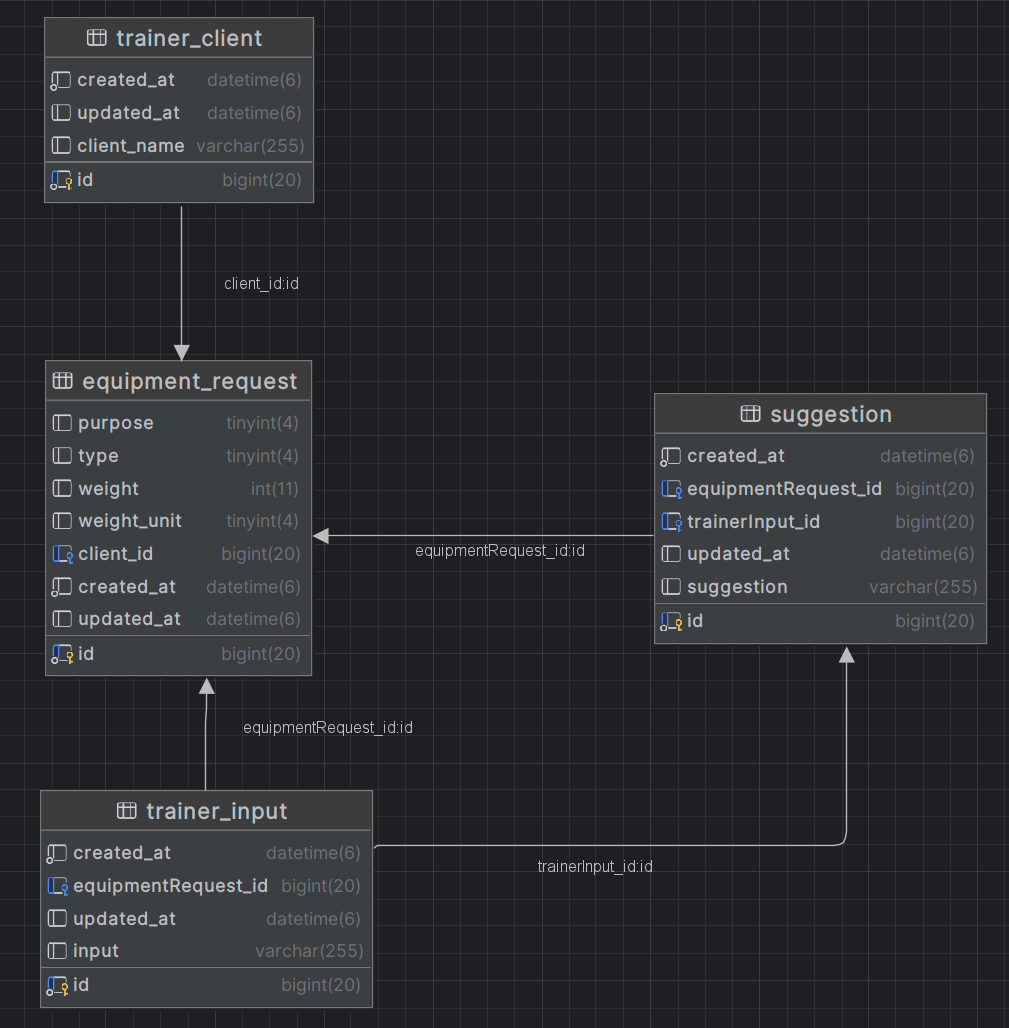
\includegraphics[scale=0.3]{images/domeinmodel}
        \caption{Formaat om data op te slaan in de databank. Een cliënt vraagt een verzoek aan om meer informatie te krijgen over een object (equipment\_request), op basis hiervan krijgt de cliënt een suggestie terug met optionele invloed van de personal trainer (trainer\_input).}
        \label{fig:domein-model}
    \end{center}
\end{figure}

\subsection{Functionaliteiten van de gebruiker}
\label{subsec:functionaliteiten-van-de-gebruiker}
Na het opzetten van het domeinmodel kunnen de bronnen voor de gebruikers gedefinieerd en geïmplementeerd worden.
Voor deze proof-of-concept is er hierbij slechts een bron blootgesteld aan de gebruiker, namelijk het doorsturen van een foto.
In de achtergrond zal de applicatie de opgevraagde gegevens en de resultaten bijhouden in de databank.
De bron stuurt de suggesties door naar de gebruiker zodat de persoon verder kan met zijn workout.
Hierbij kijkt de applicatie naar de input van de personal trainer en past het de suggesties aan waar nodig.
Belangrijk hierbij is dat de gebruiker hier geen extra input voor moet geven.

\subsubsection{Bron definiëren}
Quarkus biedt een triviale oplossing om bronnen te definiëren en bloot te stellen aan gebruikers.
Elke bron voert vervolgens enkele stappen uit, in het geval van de bron voor cliënten begint dat met het verwerken van de afbeelding.
De applicatie een verzoek naar Vertex AI met bijkomende gegevens zoals het vooraf gedefinieerde JSON-formaat.
Daarna slaat de applicatie het resultaat op in de databank en haalt het aansluitende instructies van de personal trainer op.
Met de opgevraagde gegevens omtrent de foto en eventuele bijkomende instructies van de coach zal Quarkus opnieuw een verzoek sturen naar Vertex AI om suggesties voor te stellen met behulp van generatieve AI.
Alvorens de resulterende suggesties terug te sturen naar de gebruiker zal de applicatie deze opslaan in de databank.

\subsubsection{Implementatie van de bron om suggesties te genereren}
\label{subsubsec:implementatie-bron-suggesties-genereren}
De bovenstaande bron kent de volgende uitwerking met behulp van enkele Langchain4j implementaties:
\begin{listing}[H]
    \begin{minted}[breaklines]{kotlin}
    fun getSuggestions(
        @NotNull @RestForm("image") file: File,
    ): String {
        val user = User.byName("Maurice Cantaert") ?: throw IllegalArgumentException("User can't be null")

        // 1
        val equipmentDetails = imageAnalyzer.getEquipmentDetails(file)
        val trainerInput = TrainerInput.latest(user, equipmentDetails.type)

        // 2
        equipmentDetails.client = user
        equipmentDetails.persist()

        // 3
        val response = suggestionGenerator.getSuggestion(equipmentDetails, trainerInput)
        response.persist()

        return response.suggestion
    }
    \end{minted}
    \captionof{listing}{\IfLanguageName{dutch}{Instructies van de bron om een afbeelding te analyseren en daarvoor suggesties te genereren}{Instructies of the resource to generate suggestions based on the analysed picture}}
\end{listing}
\label{code:user-resource}
Allereerst zal het systeem de gebruiker opvragen volgens de gebruikersnaam.
In de eerste stap zal daarmee de recentste input van de personal trainer voor het type fitness toestel opgevraagd worden.
Ondertussen stuurt het systeem een verzoek aan de computer visie-dienst (imageAnalyzer) om het object te analyseren.
Vervolgens, in de tweede stap, zal het systeem de resultaat van de fotoverwerker opslaan in de databank.
Ten slotte zal het systeem suggesties laten genereren door middel van een verzoek aan de generatieve AI-dienst (suggestionGenerator).

\subsubsection{Implementation van de AI-gestuurde diensten}
Zowel de imageAnalyzer als de suggestionGenerator uit codefragment~\ref{code:user-resource} maken gebruik van een eigen implementatie van Langchain4j.
Beide implementaties delen dezelfde fundamentele werking:
\begin{listing}[H]
    \begin{minted}[breaklines]{kotlin}
        UserMessage.from(
            ImageContent.from(encodedFile, mime),
            TextContent.from(
                """
            A user wants to know what fitness equipment he's looking at along with some details. Respond in the following JSON format.
            If any details are unknown (such as weight or the type), try to make an estimation.

            Answer with a single raw JSON document, WITHOUT any markdown markup such as ````json or ``` surrounding it.
            The JSON document must contain:
            - the type of equipment, such as a DUMBBELL or BARBELL, in the `type` key as a string
            - the purpose of equipment, such as STRENGTH or CARDIO, in the `purpose` key as a string
            - the weight of the equipment, in the `weight` key as a number
            - the weight measurement, either KG or LBS, in the `weight_unit` key as a string
                """.trimIndent()
            )
        )
    \end{minted}
    \captionof{listing}{\IfLanguageName{dutch}{Instructies om computer visie uit te voeren op een afbeelding om het object te analyseren en vervolgens uit te gieten in een vooraf gedefinieerd JSON-bestand}{Instructions to perform computer vision on an image to analyze the object and then pour it out into a predefined JSON file}}
\end{listing}
\label{code:get-suggestions}
Bij het oproepen van de bron beschreven in subsectie~\ref{subsubsec:implementatie-bron-suggesties-genereren} zal het systeem de functie~\textit{getEquipmentDetails()} oproepen.
Allereerst zal de dienst de afbeelding verwerken zodat deze door het systeem gebruikt kan worden voor computer visie.
Vervolgens wijst de dienst aan welk model toegepast zal worden, in dit geval is dat het Gemini 1.5 Pro model.
Het verzoek wordt verstuurd naar het model om te verwerken, zoals beschreven in codefragment~\ref{code:get-suggestions}.
Ten slotte zal de beeldverwerker het resultaat omvormen tot een gepast domeinobject dat verder gebruikt kan worden.

\subsubsection{Implementatie van de Android applicatie}
De Android-applicatie maakt gebruik van Retrofit om de bovenstaande bron op te roepen.
Door een foto uit de galerij te selecteren kan de gebruiker deze dienst oproepen.
Ten slotte geeft de app de gegenereerde suggesties weer in Markdown formaat.

\subsection{Functionaliteiten van de personal trainer uitwerken}
\label{subsec:functionaliteiten-van-de-personal-trainer-uitwerken}
Een personal trainer krijgt toegang tot twee bronnen.
Om de applicatie te gebruiken start hij met het raadplegen van de historiek van de gebruiker.
Met deze gegevens krijgt hij een globaal zicht op de vooruitgang van de gebruiker, bijvoorbeeld aan de hand van het gewicht van enkele gebruikte toestellen.
Ook krijgt hij een zicht op de hoeveelheid toestellen die gebruikt werden, hoe vaak en over welke periode.
Hiermee hoeven zowel de coach als de cliënt dit niet zelf bij te houden of te noteren.
De tweede bron bestaat uit het manipuleren van toekomstige suggesties die aan de cliënt voorgesteld zullen worden, dit aan de hand van de gegevens uit de voorgenoemde bron.
Met het toevoegen van enkele suggesties, zoals het focussen op een bepaalde oefening of meer repetities aan een lager gewicht, zal de gebruiker gepersonaliseerde suggesties krijgen bij het volgende gebruik van de Android app.
Bovendien zal de coach deze gegevens niet zelf nog bij te houden, deze zullen telkens raadpleegbaar blijven in de databank bij volgende consultaties.

\subsubsection{Implementatie}
De implementatie van de voorgaande functionaliteit voor gebruikers haalt reeds de invoer op van de personal trainer.
Langchain4j krijgt deze invoer en zorgt ervoor dat Vertex AI hier rekening mee houdt.
Het definiëren van de bron en de manipulatie van de data in de databank is gelijkaardig met~\nameref{subsec:functionaliteiten-van-de-gebruiker}.
De personal trainer kan deze bronnen oproepen door middel van Postman, een platform voor het rechtstreeks gebruiken van achterliggende API's.
Het is mogelijk om een externe applicatie zoals een website of desktop applicatie te maken met een gebruiksvriendelijke interface, dit valt echter buiten de scope van deze proof-of-concept.

\subsection{Opmerkingen}
\label{subsec:opmerkingen}
Tijdens het uitwerken van de proof-of-concept kwamen enkele uitdagingen aan bod:
\begin{itemize}
    \item De automatische integratie van \textbf{Quarkus AI} met Langchain4j zorgt momenteel voor enkele problemen bij het uitvoeren van correcte computer visie.
    Een mogelijke oorzaak is het foutief verwerken van de afbeelding om door te sturen naar het Gemini taalmodel, waardoor sommige verwerkingen minder accuraat zijn.
    Om dit te mitigeren is dit deel van de proof-of-concept zonder Quarkus AI geschreven in pure Langchain4j instructies.
    Hiermee zijn de resultaten zoals verwacht en overeenkomstig met de resultaten in de voorafgaande testen.
    \item De \textbf{vooraf gedefinieerde instructies} zoals beschreven in codefragement~\ref{code:get-suggestions} vereisen specifieke voorwaarden om een gepast resultaat te bekomen.
    Hierbij moet de achterliggende service enkele zaken verduidelijken, zoals het gevraagde JSON-formaat of de context van het verzoek.
\end{itemize}

\section{Reproduceren van de proof-of-concept}
\label{sec:reproduceren-van-de-proof-of-concept}
Om het reproduceren van deze proof-of-concept mogelijk te maken is er een Gradle-scripts die uitgevoerd kan worden om de applicatie op te starten.
Belangrijk hierbij is dat er een~\nameref{subsec:docker} omgeving aanwezig is en draait, zodat Quarkus een test databank kan genereren.
Bovendien is het belangrijk om een~\textit{.env} bestand aan te maken in de kernmap van het project met volgende waarden om de Gemini omgeving op te kunnen roepen:
\begin{listing}[H]
    \begin{minted}[breaklines]{properties}
GEMINI_PROJECT_ID=rare-nectar-414417
GEMINI_PROJECT_LOCATION=europe-west1
    \end{minted}
    \captionof{listing}{\IfLanguageName{dutch}{Omgevingswaarden met informatie over Gemini}{Environment values with information reegarding Gemini}}
\end{listing}

\section{Resultaten}
\label{sec:resultaten}
De uitwerking van de proof-of-concept heeft een gunstig resultaat.
Cliënten kunnen makkelijk suggesties opvragen op basis van ingezonden afbeeldingen zonder bijkomende invoer.
Deze suggesties worden in Markdown formaat getoond op de telefoon van de gebruiker om een gepast overzicht te krijgen.
De historiek van de gebruiker wordt bijgehouden en is ten alle tijde raadpleegbaar door de personal trainer.
Bovendien kan de personal trainer volgende suggesties manipuleren door middel van eigen invoer in te geven.
In subsectie~\ref{subsec:opmerkingen} komen enkele opmerkingen aan bod.